\section{Excluded Federal Courts}
\label{app:courts}
CourtListener assigns federal jurisdiction codes to many bodies beyond the
fourteen courts in the population. Every excluded court is listed in the released
artefact \texttt{01\_courts.json}. They fall into four groups: the historical
circuit courts that sat before the Judiciary Act of 1891, appearing under roughly
130 identifiers of the form \texttt{circt*}; abolished or specialized Article I
and Article III courts, among them the Court of Customs and Patent Appeals, the
Court of Claims, and the Court of International Trade; the Foreign Intelligence
Surveillance Court and its Court of Review; and administrative review bodies
whose decisions are published alongside judicial opinions, among them the Board
of Immigration Appeals, the Merit Systems Protection Board, and the Patent Trial
and Appeal Board.

Excluding administrative bodies is a substantive choice. Agency adjudicators use
the same vocabulary of non-resolution, but they are not courts of appeals, their
decisions carry different precedential force, and the citation practices layer
two depends on differ. The historical circuit courts are excluded for a different
reason: their reporting is uneven and their text largely OCR-derived, so a rate
computed over them would measure digitization as much as judicial practice.

\section{Text Extraction}
\label{app:text}

CourtListener stores an opinion's text in whichever markup flavours its upstream
sources supplied. We take the first field with usable content in the order
\texttt{html\_columbia}, \texttt{html\_lawbox}, \texttt{xml\_harvard},
\texttt{html\_anon\_2020}, \texttt{html}, \texttt{plain\_text},
\texttt{html\_with\_citations}. The citation-annotated variant is last because it
injects anchor text into the body. Markup is removed by closing block-level tags
into newlines, deleting remaining tags, unescaping entities, and normalizing
whitespace; character offsets in the released benchmark refer to this normalized
text. Table \ref{tab:textsrc} reports which field supplied the text, by period.
Source composition shifts with period because different digitization projects
covered different eras, which is one reason we report period-stratified rates
rather than a single pooled trend.

\IfFileExists{generated/tab_textsrc_full.tex}{\begin{table*}[t]
\centering\small
\begin{tabular}{lrrrr}
\toprule
field & pre-1990 & 1990-2004 & 2005-2014 & 2015-2026  \\
\midrule
\texttt{html} & 17.2 & 30.1 & 2.3 & 0.0 \\
\texttt{html\_lawbox} & 10.5 & 0.6 & 12.9 & 0.0 \\
\texttt{plain\_text} & 0.0 & 13.3 & 16.8 & 67.7 \\
\texttt{xml\_harvard} & 72.3 & 56.0 & 68.0 & 32.3 \\
\bottomrule
\end{tabular}
\caption{Text source field by period, as a percentage of eligible opinions in that period.}
\label{tab:textsrc}
\end{table*}
}{}


\section{The Frozen Trigger Dictionary}
\label{app:dict}

Figure \ref{fig:trigger} lists the thirteen expressions with
their corpus frequencies. The regular expressions themselves are reproduced
below; they were fixed before annotation and their SHA-1 is \texttt{\DictSHA}.

\IfFileExists{generated/tab_regex_full.tex}{\begin{figure*}[t]
\centering\scriptsize
\begin{verbatim}
T01  need(?:s|ed)?\s+not\s+(?:\w+\s+){0,2}?decide\b
T02  need(?:s|ed)?\s+not\s+(?:\w+\s+){0,2}?reach\b
T03  \bdo(?:es)?\s+not\s+(?:\w+\s+){0,2}?decide\b
T04  \bdo(?:es)?\s+not\s+(?:\w+\s+){0,2}?reach\b
T05  declin(?:e|es|ed|ing)\s+to\s+(?:\w+\s+){0,2}?decide\b
T06  declin(?:e|es|ed|ing)\s+to\s+(?:\w+\s+){0,2}?address\b
T07  \bwithout\s+deciding\b
T08  \bassuming\s+(?:\w+\s+){0,4}?without\s+deciding\b
T09  assum(?:e|es|ed)\s+(?:\w+\s+){0,4}?without\s+deciding\b
T10  express(?:es|ed|ing)?\s+no\s+(?:\w+\s+){0,2}?opinion\b
T11  reserv(?:e|es|ed|ing)\s+(?:\w+\s+){0,3}?(?:question|questions|issue|issues|matter|judgme
    nt|decision)\b|reserv(?:e|es|ed|ing)\s+(?:\w+\s+){0,3}?for\s+another\s+(?:day|case)\b
T12  leav(?:e|es|ing)\s+(?:\w+\s+){0,4}?(?:for|to|until)\s+another\s+(?:day|case|occasion)\b
T13  \b(?:not|un)\s*necessary\s+to\s+(?:decide|reach|resolve|address)\b
\end{verbatim}
\caption{The thirteen frozen expressions as regular expressions, matched case-insensitively over whitespace-normalized text.}
\label{tab:regex}
\end{figure*}
}{}


T08 and T09 are proper subsets of T07 by construction. They are retained because
the design names them separately, and a passage matching several expressions is
counted once in opinion-level rates while keeping every identifier. T11 is the
only expression not matched as written, for the reason given in
\S\ref{sec:prev}.

\section{Issue Statement Extraction}
\label{app:issue}

An item needs a statement of the proposition at stake that does not reveal the
answer. We derive it from the sentence containing the anchor rather than from a
fixed character budget, which stops the clause running into whatever the court
said next.

The procedure takes the material following the anchor within the anchor's
sentence, deletes reporter citations and signals, and looks for a
\emph{whether}-complement within the first sixty characters. If none is present
but the clause opens with a complementizer or a preposition taking a
propositional object, it is rewritten as a \emph{whether}-clause. If it opens
with neither, it is kept as a noun phrase, but only when its first token is not a
verb, negation, conjunction, or pronoun, since those signal a fragment rather
than a statement of an issue. Where the trigger closes its own sentence, the
material before the anchor is used instead, and only when that material itself
names the issue with \emph{whether}, \emph{the question of}, or \emph{the issue
of}. Two filters run last. Any dictionary expression or holding cue in the
candidate statement is cut, which is what allows the claim that no issue
statement contains one, and statements with fewer than three content words, or
more than forty percent non-alphabetic, are rejected as extraction debris.

Rejection is not random. An anchor with no extractable issue statement does not
enter the frame, so the benchmark is a sample of anchors with a recoverable
proposition rather than of all anchors. Table \ref{tab:extract} reports the yield
by expression and by court so that the direction of any bias is visible.

\IfFileExists{generated/tab_extract_full.tex}{\begin{table}[t]
\centering\small
\begin{tabular}{lrrr}
\toprule
id & anchors & with issue & yield (\%) \\
\midrule
T01 & 49,640 & 34,951 & 70.4 \\
T02 & 30,909 & 16,737 & 54.1 \\
T03 & 22,309 & 15,820 & 70.9 \\
T04 & 45,401 & 25,678 & 56.6 \\
T05 & 8,144 & 5,871 & 72.1 \\
T06 & 21,004 & 10,165 & 48.4 \\
T07 & 30,894 & 23,189 & 75.1 \\
T08 & 4,718 & 3,420 & 72.5 \\
T09 & 7,779 & 5,663 & 72.8 \\
T10 & 24,641 & 17,710 & 71.9 \\
T11 & 34,080 & 15,684 & 46.0 \\
T12 & 3,508 & 1,826 & 52.1 \\
T13 & 18,876 & 11,670 & 61.8 \\
\bottomrule
\end{tabular}
\caption{Issue-statement extraction yield by expression.}
\label{tab:extract}
\end{table}
}{}


\section{Annotation Guidelines}
\label{app:guide}

The guidelines below are reproduced verbatim from the frozen protocol. Version
1.0 was drafted before the pilot; version 1.1 incorporates the single revision
the design permits, made once after the pilot and before any main-sample
annotation.

\begin{quote}\scriptsize\begin{verbatim}
TASK. You are given a legal issue and a passage from
  a United States federal
appellate opinion. Decide whether the opinion
  resolved that issue.

LABELS.
  DECIDED     The authoring court resolved the
    issue. It stated a holding, a
              conclusion, or a
                determination on the
                issue, whether or not
                that
              resolution was necessary
                to the judgment, and
                whether or not it
              was later characterized
                as dictum.
  UNRESOLVED  The authoring court did not resolve
    the issue for itself.

If and only if the label is UNRESOLVED, assign one
  sublabel.
  AVOIDED     The court declined to reach the
    issue because some other ground
              disposed of the case or
                the claim. Typical
                form: "because we
              affirm on qualified
                immunity grounds, we
                need not decide
                whether
              the search was lawful."
  ASSUMED     The court proceeded on a stated
    assumption about the issue and
              resolved the case on
                other grounds, so that
                the assumption did
              no independent work.
                Typical form:
                "assuming without
                deciding
              that the statute reaches
                this conduct, the
                evidence is
              insufficient."
  RESERVED    The court expressly held the issue
    open for future resolution,
              signalling that it
                remains available.
                Typical form: "we
                leave for
              another day whether
                Chevron survives in
                this context."

DECISION RULES.
  L1-1  ATTRIBUTION. The label describes what THIS
    opinion did. Language about
        what a different court did, whether
          a lower court, a sister circuit,
          or
        the Supreme Court, does not by
          itself make this opinion's
          disposition
        UNRESOLVED. "The district court
          concluded it need not decide X"
          tells
        you about the district court. Read
          on to see what this court did.
  L1-2  UNIT. In a cluster containing a majority
    opinion and separate opinions,
        each opinion is its own unit. A
          dissent that would decide an issue
          the
        majority avoided is DECIDED for the
          dissent and UNRESOLVED for the
        majority.
  L1-3  LATER RESOLUTION CONTROLS. A court may
    write "we need not decide X" and
        then decide X anyway, in the same
          opinion, in an alternative
          holding, in
        a footnote, or in a later section.
          Where the opinion does resolve the
        issue somewhere, the label is
          DECIDED. A court's
          characterization of
        what it need not do controls only
          where no independent resolution
        follows.
  L1-4  ASSUMPTION THAT DOES WORK. If the court
    assumes a proposition and the
        assumption is then treated as
          settled for the remainder of the
          analysis
        in a way that determines the
          outcome, the label remains
          UNRESOLVED and
        the sublabel is ASSUMED. Assuming a
          proposition is not deciding it,
          even
        when the assumption drives the
          result.
  L1-5  NO TRIGGER REQUIRED. UNRESOLVED does not
    require any particular phrase.
        A court can leave an issue open in
          ordinary prose.
  L1-6  PARTIAL RESOLUTION. The unit is the
    proposition named in the issue
        statement, not the broader legal
          question it belongs to. If the
          court
        resolves the anchored proposition
          but leaves a neighbouring one
          open,
        the label is DECIDED. If the court
          resolves a neighbouring
          proposition
        but leaves the anchored one open,
          the label is UNRESOLVED.
  L1-7  REMANDS. An issue remanded for the
    district court to address in the
        first instance is UNRESOLVED,
          sublabel AVOIDED, unless the
          appellate
        court also states the governing rule
          and applies it.
  L1-8  ABSTAIN. If the passage is too corrupt,
    too truncated, or too ambiguous
        to support either label, output
          UNCLEAR rather than guessing.
  L1-9  ISSUES THIS OPINION NEVER TAKES UP.
    Sometimes the only reason an issue
        is in front of you is that the
          opinion mentioned, in a
          parenthetical or
        in a description of some other
          court's work, that a different
          court did
        not decide it, and this opinion
          never reaches the issue in its own
        right. That is neither DECIDED nor
          UNRESOLVED for this opinion.
          Output
        UNCLEAR. This rule does not apply
          where the opinion goes on to
          engage
        with the issue itself: there, L1-1
          and L1-3 govern.
\end{verbatim}\end{quote}

\noindent Version 1.1. The single permitted revision after the pilot, and the layer-two and issue-statement guidelines, are in the released package.


\section{Pilot Study and Protocol Revision}
\label{app:pilot}

The pilot ran on a preliminary frame built from a leading portion of the bulk
opinion table, before the full pass was committed to. Its purpose was to find
out whether the guideline could be applied at all, whether the controls behaved,
and which strata were worth sampling heavily. Sixty items were annotated. Pilot
items are not part of the benchmark and no pilot label appears in any result.

\subsection{What the pilot showed} Labels fell out by stratum as follows:
\textsc{ctrl\_hold} 12 \textsc{decided} and 0 \textsc{unresolved};
\textsc{plain} 19 \textsc{unresolved} and 1 \textsc{decided};
H2 8 \textsc{unresolved} and 2 \textsc{decided};
H1 5 \textsc{unresolved}, 5 \textsc{decided}, and 5 \textsc{unclear}.

Three things follow. The holding-cue control behaves as intended and is not
contaminated. The \textsc{plain} stratum is nearly degenerate: a trigger with no
structural complication almost always does mean the court left the issue open,
which is why a keyword rule scores as well as it does and why that score means
little. The H1 stratum is close to an even split, so it is where the task
actually lives, and the sample was reallocated toward it. This reallocation
changes only how many items are drawn per stratum. Label definitions and stratum
definitions were fixed before the pilot and held throughout.

\subsection{The one protocol revision} Version 1.0 of the guideline had no rule
for a passage whose only trigger sits inside a parenthetical or a description of
another court's work, on a question the present opinion never reaches in its own
right. A citation noting that the Supreme Court declined to decide whether an
airport user fee was excessive tells you nothing about the disposition of the
Federal Circuit opinion that cites it, and forcing a choice between
\textsc{decided} and \textsc{unresolved} would have manufactured a label. Rule
L1-9 routes these to \textsc{unclear}. It uses an existing label; it adds none.
This is the single revision the design permits, it was made once, before any
main-sample annotation, and the changelog is reproduced in
Appendix~\ref{app:guide}.

\subsection{Three pipeline defects the pilot exposed} These concern candidate
construction, not the guideline. The pattern flagging a trigger as plausibly
describing another institution was case-sensitive, matching ``the district
court'' but missing ``the District Court,'' which appellate opinions write about
as often; it now also recognizes ``the court held'' and its near neighbours. The
annotator was shown a later holding sentence only for items already flagged H2,
though Rule L1-3 turns on precisely that passage, so an H1 item whose opinion
later resolved the issue was unanswerable rather than hard; the sentence is now
shown whenever one exists outside the displayed window. And ``our holding'' was
a control locator, but in the pilot it pointed at a named prior case rather than
the present disposition every time it fired, so it was dropped.

\subsection{What the pilot did not do} It was not used to adjust any label
boundary. The trigger dictionary was frozen before the pilot and is unchanged;
in particular, the pilot surfaced two recurring dictionary false positives, and
neither was patched. One is the statutory-scope reading of \emph{reach}, as in
``the shipment clause does not reach shipments between the continental States,''
which is a holding about a statute rather than a non-resolution. The other is a
line-break artefact in the source text that splits \emph{preserving} into
\texttt{P} and \texttt{reserving}, which then matches T11. Both stay in, are
labelled \textsc{decided} by the guideline, and are counted against the
dictionary in \S\ref{sec:models}.


\section{Dictionary Recall Audit}
\label{app:recall}

The frozen dictionary bounds what candidate generation can find. It says nothing
about non-resolution expressed in language outside it. To bound that, we drew a
random sample of eligible opinions containing no dictionary expression and read
them for issues the court discussed and left unresolved.

Reading whole opinions at random is a weak audit. A non-resolution can sit
anywhere in forty pages, most opinions contain none, and an annotator who has
internalized the dictionary is primed to see the vocabulary it already
covers.

We use a second, deliberately wider probe list instead. Fifteen expressions
outside the frozen dictionary were written after the fact and run over a random
sample of \RecallSampled{} opinions the dictionary called clean. The probe is
confined to this audit and enters neither candidate generation, the benchmark,
nor any prevalence figure.

\RecallHit{} of clean opinions contain at least one probe expression. Table
\ref{tab:recall} gives the breakdown. What that figure bounds needs stating
carefully. It is a measure of \emph{lexical} coverage, not of missed
non-resolution. Some probe hits are genuine, as in a Seventh Circuit opinion
that writes ``Volkswagen does not raise this argument and we do not resolve
it,'' and then says the question ``remains unsettled.'' Others are the same
statutory-scope reading of \emph{reach} and \emph{address} that already
contaminates the frozen dictionary, where the court is saying what a statute
covers rather than what it declined to decide. Annotating a sample of probe hits would be needed to convert the probe rate
into an estimate of missed non-resolution, so we report it as a coverage
figure.

The largest omission is the \emph{address}, \emph{consider}, \emph{resolve}
family. The frozen dictionary contains \emph{need not decide} and \emph{need not
reach} but not \emph{need not address}, and \emph{decline to address} but not
\emph{decline to consider}. The design named thirteen expressions and they were
frozen before annotation, so the gap stands rather than being patched. The pilot
had already flagged one instance, in a control opinion reading ``we need not
address the government's contention'' that was nonetheless admitted to the
zero-trigger pool.

Two consequences follow for how the paper's numbers should be read. Population
prevalence in \S\ref{sec:prev} measures explicitly marked non-resolution using
one fixed vocabulary, and a wider vocabulary would find more, so it is a floor
rather than an estimate of the phenomenon. And the control pool is contaminated
in a known direction, since some opinions admitted as trigger-free do contain
unresolved issues expressed in language outside the dictionary. That
contamination makes the controls harder rather than easier, so it works against
every reported separation rather than for it.

\IfFileExists{generated/tab_recall_full.tex}{\begin{table*}[t]
\centering\footnotesize
\begin{tabular}{llrr}
\toprule
id & probe expression & $n$ & \% of clean \\
\midrule
P01 & need not address & 128 & 3.20 \\
P02 & need not consider & 92 & 2.30 \\
P03 & need not resolve & 46 & 1.15 \\
P04 & no occasion to decide & 14 & 0.35 \\
P05 & leave open the question & 45 & 1.12 \\
P06 & decline to consider/resolve/reach & 80 & 2.00 \\
P07 & assume arguendo & 111 & 2.77 \\
P08 & we may assume & 44 & 1.10 \\
P09 & pretermit & 18 & 0.45 \\
P10 & do not address/consider/resolve & 254 & 6.35 \\
P12 & for purposes of this appeal we assume & 1 & 0.03 \\
P13 & intimate no view & 9 & 0.22 \\
\bottomrule
\end{tabular}
\caption{Probe expressions found in opinions the frozen dictionary called clean. The probe was written after the fact and is used only for this audit.}
\label{tab:recall}
\end{table*}
}{}




\section{Full Prevalence Tables}
\label{app:prev}

\begin{table*}[t]\centering\small
\begin{tabular}{lrrrr}
\toprule
court & 1990-2004 & 2005-2014 & 2015-2026 & pre-1990 \\
\midrule
Supreme Court & 28.88 & 30.96 & 34.35 & 14.78 \\
1 Cir. & 28.67 & 31.66 & 39.27 & 19.87 \\
2 Cir. & 25.66 & 19.77 & 28.40 & 15.42 \\
3 Cir. & 34.48 & 21.23 & 25.60 & 20.21 \\
4 Cir. & 12.30 & 11.62 & 11.85 & 13.00 \\
5 Cir. & 22.07 & 20.69 & 20.02 & 15.01 \\
6 Cir. & 14.63 & 24.52 & 26.73 & 10.87 \\
7 Cir. & 19.80 & 16.86 & 18.77 & 17.33 \\
8 Cir. & 17.43 & 19.17 & 18.60 & 12.82 \\
9 Cir. & 20.24 & 17.72 & 21.17 & 18.68 \\
10 Cir. & 21.11 & 27.65 & 32.08 & 12.23 \\
11 Cir. & 28.97 & 19.78 & 23.54 & 24.72 \\
D.C. Cir. & 29.92 & 25.94 & 32.50 & 19.18 \\
Fed. Cir. & 16.59 & 20.22 & 24.93 & 17.89 \\
\bottomrule
\end{tabular}
\caption{Share of opinions containing at least one dictionary expression, by court and period.}\label{tab:cp}
\end{table*}

\begin{table}[t]\centering\small
\begin{tabular}{lrrr}
\toprule
type group & $N$ & $k$ & \% \\
\midrule
majority/lead & 864,804 & 169,373 & 19.59 \\
other & 1,664 & 101 & 6.07 \\
separate & 61,786 & 6,136 & 9.93 \\
\bottomrule
\end{tabular}
\caption{By opinion type.}\label{tab:type_group}
\end{table}

\begin{table}[t]\centering\small
\begin{tabular}{lrrr}
\toprule
precedential status & $N$ & $k$ & \% \\
\midrule
Errata & 104 & 3 & 2.88 \\
Published & 767,586 & 160,008 & 20.85 \\
Relating-to & 552 & 21 & 3.80 \\
Unknown & 3,291 & 1,139 & 34.61 \\
Unpublished & 156,706 & 14,439 & 9.21 \\
\bottomrule
\end{tabular}
\caption{By precedential status.}\label{tab:precedential_status}
\end{table}


\begin{figure}[t]
\centering
\IfFileExists{generated/fig_heat.pdf}{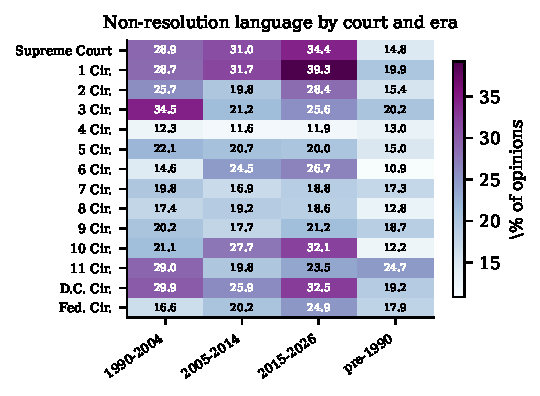
\includegraphics[width=\columnwidth]{generated/fig_heat.pdf}}{}
\caption{Share of eligible opinions containing at least one frozen dictionary
expression, by court and period. Cells with fewer than 150 eligible opinions are
left blank rather than plotted as noise.}
\label{fig:heat}
\end{figure}

\section{Cross-Check Against the Search Index}
\label{app:api}

The bulk release and the public CourtListener search index are built from the
same database but refreshed on different schedules and tokenized differently.
Querying the index for the thirteen literal phrases, restricted to the fourteen
courts, gives an estimate of how many opinions contain each expression that is
independent of our text extraction, markup handling, and field precedence.

Three hundred count queries were issued against the v4 search endpoint: a
denominator for each of the fourteen courts, a denominator for each court and
period, and a count for each of the thirteen literal phrases, both per court and
pooled. No opinion text was retrieved.

Two differences from the bulk pipeline are expected and neither is a defect.
The index counts opinions as the search system stores them, while our
denominator counts opinions surviving the eligibility criteria of
\S\ref{sec:corpus}, which remove short orders and duplicates; the index
denominator is therefore the larger of the two. And the index matches literal
phrases, while the frozen dictionary tolerates a few intervening words and
constrains T11, so the two counts are not measuring the same event. The
comparison is useful precisely because the two disagree in known directions: a
large unexplained gap would indicate that markup handling or field precedence
was losing text, and a close match on the shape of the distribution across
courts and expressions indicates that it is not.

The pooled index count over the thirteen literal phrases restricted to the
fourteen courts is 108{,}669 opinions against a denominator of
\ApiTotal{} indexed opinions, an implied rate of 7.8\%. Ranking the expressions
by frequency, the index and the bulk corpus agree on the ordering of the top
group, with \emph{need not decide} first in both.

\IfFileExists{generated/tab_api_full.tex}{\begin{table*}[t]
\centering\small
\begin{tabular}{lr}
\toprule
court & indexed opinions \\
\midrule
Supreme Court & 498,145 \\
1 Cir. & 37,036 \\
2 Cir. & 88,338 \\
3 Cir. & 65,415 \\
4 Cir. & 66,616 \\
5 Cir. & 117,894 \\
6 Cir. & 62,972 \\
7 Cir. & 71,787 \\
8 Cir. & 79,172 \\
9 Cir. & 137,966 \\
10 Cir. & 40,431 \\
11 Cir. & 53,966 \\
D.C. Cir. & 40,448 \\
Fed. Cir. & 28,090 \\
\bottomrule
\end{tabular}
\caption{Denominators reported by the CourtListener search index, used only for the cross-check in Appendix~\ref{app:api}.}
\label{tab:api}
\end{table*}
}{}



\section{Supplementary Tables}
\label{app:supp}
\IfFileExists{generated/tab_context_full.tex}{\input{generated/tab_context_full}}{}

\IfFileExists{generated/tab_prev_period_full.tex}{\input{generated/tab_prev_period_full}}{}

\IfFileExists{generated/tab_paths_full.tex}{\input{generated/tab_paths_full}}{}

\IfFileExists{generated/tab_tailpair_full.tex}{\begin{table*}[t]
\centering
\begin{minipage}[t]{0.46\textwidth}
\centering\small
\begin{tabular}{lrr}
\toprule
split & $n$ & \% unresolved \\
\midrule
COURT & 54 & 57.4 \\
DEV & 143 & 53.8 \\
TEMPORAL & 44 & 54.5 \\
TEST & 123 & 54.5 \\
\bottomrule
\end{tabular}
\captionof{table}{Evaluation splits. They are disjoint at the opinion level and only \textsc{dev} was used for fitting.}
\label{tab:splits}
\end{minipage}\hfill
\begin{minipage}[t]{0.50\textwidth}
\centering\small
\begin{tabular}{lrr}
\toprule
stratum & $n$ & agreement with full context (\%) \\
\midrule
CTRL\_HOLD & 4 & 75.0 \\
H1 & 11 & 81.8 \\
H2 & 7 & 100.0 \\
PLAIN & 9 & 100.0 \\
\bottomrule
\end{tabular}
\captionof{table}{How often the annotator's sentence-only label matches the label the same annotator gave with the full window. A within-annotator context ablation, not an inter-annotator statistic.}
\label{tab:humanabl}
\end{minipage}
\end{table*}
}{\IfFileExists{generated/tab_splits_full.tex}{\begin{table*}[t]
\centering\small
\begin{tabular}{lrr}
\toprule
split & $n$ & \% unresolved \\
\midrule
COURT & 54 & 57.4 \\
DEV & 143 & 53.8 \\
TEMPORAL & 44 & 54.5 \\
TEST & 123 & 54.5 \\
\bottomrule
\end{tabular}
\caption{Evaluation splits. They are disjoint at the opinion level and only \textsc{dev} was used for fitting.}
\label{tab:splits}
\end{table*}
}{}
\IfFileExists{generated/tab_humanabl_full.tex}{\begin{table}[t]
\centering\small
\begin{tabular}{lrr}
\toprule
stratum & $n$ & agreement with full context (\%) \\
\midrule
CTRL\_HOLD & 4 & 75.0 \\
H1 & 11 & 81.8 \\
H2 & 7 & 100.0 \\
PLAIN & 9 & 100.0 \\
\bottomrule
\end{tabular}
\caption{How often the annotator's sentence-only label matches the label the same annotator gave with the full window. A within-annotator context ablation, not an inter-annotator statistic.}
\label{tab:humanabl}
\end{table}
}{}
}

These are collected rather than placed inline because each is a secondary cut on
a quantity already reported.

\section{Model Details}
\label{app:models}

\subsection{Context conditions} Every system is evaluated under four windows
around the anchor: the anchor's sentence (\textsc{sent}), and $\pm256$,
$\pm1024$, and $\pm4096$ characters. Windows are cut from the normalized text and
whitespace-collapsed. The sentence condition isolates local lexical evidence; the
widest condition is the only one that routinely reaches a later holding sentence
in the same opinion, which is what the H2 stratum requires.

\subsection{Lexical rule} The floor. The frozen dictionary is applied to the
context window and the item is predicted \textsc{unresolved} when any expression
matches. This is not a strawman: it is exactly the procedure that generated the
candidates, and it is what a keyword system would do. Because controls are drawn
from opinions containing no dictionary expression anywhere, the rule is close to
perfect on the \textsc{ctrl} strata by construction, and its overall number is
therefore an optimistic reading of what phrase matching achieves. The strata that
matter are H1 and H2, where the rule is wrong whenever the annotation says the
court's actual disposition runs against the phrase.

\subsection{Sparse baseline} TF-IDF over word unigrams and bigrams, minimum
document frequency two, at most 60{,}000 features, sublinear term frequency,
followed by $\ell_2$-regularized logistic regression with $C=4$ and balanced
class weights. Trained on \textsc{dev} only.

\subsection{Encoders} LEGAL-BERT \citep{chalkidis2020legalbert} and
DistilRoBERTa, fine-tuned for five epochs at learning rate $2\times10^{-5}$,
batch size 16, maximum length 512 tokens, with the issue statement as the first
segment and the context window as the second, truncating only the context.
Class weights are inverse to \textsc{dev} frequency. The 512-token cap means the
$\pm4096$ condition is truncated for these models, so their context curve
understates what a long-context architecture could use; this is stated in the
Limitations.

\subsection{Leakage control} A classifier trained on the issue statement alone,
with no context at all. Issue statements are constructed to be neutral and any
dictionary expression or holding cue is cut from them, so this classifier should
sit near the majority-class baseline. It is the check on how much of the
benchmark is answerable from the phrasing of the issue alone.

\subsection{Uncertainty} Macro-$F_1$ intervals are percentile bootstrap over
2{,}000 resamples of the evaluation set. Each item comes from a distinct opinion,
so resampling items and resampling opinions coincide here; the clustered
bootstrap is needed only in \S\ref{sec:long}, where several citing passages can
share an origin.

\subsection{Splits} The four evaluation conditions are disjoint and nested in a
fixed order. Every item from the two reserved courts forms \textsc{court}. Of
what remains, every item filed in \TemporalCut{} or later forms
\textsc{temporal}. The remainder is split at random into \textsc{test} and
\textsc{dev}, and \textsc{dev} is the only portion any system was fit on. The
hard-negative subset is not a split: it cuts across all of them, and is reported
as a breakdown.

\IfFileExists{generated/tab_stratum_acc_full.tex}{\begin{table*}[t]
\centering\small
\begin{tabular}{llrrr}
\toprule
stratum & context & $n$ & lexical & TF-IDF \\
\midrule
CTRL\_HOLD & SENT & 44 & 1.000 & 0.750 \\
CTRL\_HOLD & W1024 & 44 & 1.000 & 0.318 \\
CTRL\_HOLD & W256 & 44 & 1.000 & 0.545 \\
CTRL\_HOLD & W4096 & 44 & 1.000 & 0.227 \\
CTRL\_RAND & SENT & 9 & 1.000 & 0.222 \\
CTRL\_RAND & W1024 & 9 & 1.000 & 0.556 \\
CTRL\_RAND & W256 & 9 & 1.000 & 0.444 \\
CTRL\_RAND & W4096 & 9 & 1.000 & 0.333 \\
H1 & SENT & 38 & 0.895 & 0.947 \\
H1 & W1024 & 38 & 0.895 & 0.816 \\
H1 & W256 & 38 & 0.895 & 0.947 \\
H1 & W4096 & 38 & 0.895 & 0.842 \\
H2 & SENT & 43 & 0.907 & 0.907 \\
H2 & W1024 & 43 & 0.907 & 0.814 \\
H2 & W256 & 43 & 0.907 & 0.930 \\
H2 & W4096 & 43 & 0.907 & 0.814 \\
PLAIN & SENT & 52 & 0.942 & 0.962 \\
PLAIN & W1024 & 52 & 0.942 & 0.885 \\
PLAIN & W256 & 52 & 0.942 & 0.923 \\
PLAIN & W4096 & 52 & 0.942 & 0.865 \\
\bottomrule
\end{tabular}
\caption{Accuracy by stratum and context width. The lexical rule is the frozen dictionary applied to the window.}
\label{tab:stratacc}
\end{table*}
}{}


\subsection{Zero-shot language model}
\LLMName{} (revision \texttt{\LLMRevision}) runs on one \LLMDevice{} with
unquantized \LLMDtype{} weights. Logits are cast to float32 before scoring.
Nothing is generated: for each item we form one prompt and compare the summed
log-probability of the continuation
\texttt{ DECIDED} against \texttt{ UNRESOLVED}. Scoring rather than generating
removes refusals, verbose answers needing parsing, and format drift that varies
with prompt length, all of which would otherwise be confounded with difficulty.
Prompts truncate to 1600 tokens, which binds only in the widest condition. The
prompt is fixed across conditions and reads, in full: a one-line framing that the
passage is from a United States federal appellate opinion, the issue, the
passage, and the question whether the court resolved that issue or left it
unresolved, answerable in one word. No few-shot examples are supplied and the
annotation guideline is not shown, so the model sees strictly less than the
annotator did.

\IfFileExists{generated/tab_llmstratum_full.tex}{\input{generated/tab_llmstratum_full}}{}



\section{Judicial Characterizations and Layer Two}
\label{app:layer2}
\label{app:judicial}
One annotator produced the study's labels. This appendix reports a check built
from a source no annotator touched, and the citation machinery behind
\S\ref{sec:long}.

\subsection{Judges label each other's opinions}
When a court writes ``\emph{Smith}, 123 F.3d 456, 460 (declining to decide
whether the statute applies),'' it asserts on the record that \emph{Smith} did
not resolve that question; ``(holding that \dots)'' asserts the opposite. We
scanned all \NEligible{} eligible opinions for reporter citations and applied a
frozen two-class characterization dictionary to a window around each.
\NCharLoose{} passages matched, but the loose form is unreliable: a marker near a
citation is often about something else, as where ``it did not reach a verdict''
refers to a jury. Requiring the verb to bind directly to the citation, as a
parenthetical or appositive, leaves \NCharTight{} passages, \NCharLZero{} of them
assertions of non-resolution, over \NCharOps{} cited opinions. We release this
set.

\subsection{Why it cannot validate the annotations}
The obvious use fails. Suppose a later court says \emph{Smith} held $X$ and our
annotation says \emph{Smith} left $X$ open. Two explanations fit: our label is
wrong, or the later court has overstated \emph{Smith}, which is the phenomenon
this paper measures. Nothing in the disagreement distinguishes them. We report
this because the design is tempting and the flaw shows only once the numbers are
in front of you.

\subsection{Proximity matching and why it failed}
Pairing each characterization with the sentence in the cited opinion sharing the
most content words gives \NJudgeBench{} items (\NJudgeUnres{} unresolved,
\NJudgeDec{} decided), but systems transfer poorly: the frozen dictionary reaches
\JudgeLexF{} macro-$F_1$ against 0.946 on the annotated benchmark. The cause is
measurable and is not the labels. Among items a judge called unresolved, only
8.2\% carry a dictionary expression in the selected anchor sentence, against
0.5\% of items a judge called decided: enriched sixteenfold, so the labels carry
signal, but in more than nine cases in ten the matcher selects where the opinion
\emph{discusses} the issue rather than where it \emph{disposes} of it. Accuracy
rises monotonically with match quality, from 0.485 to 0.610, the pattern
anchoring noise predicts and label noise does not. Asking instead whether a
dictionary expression sits within 400 characters of the characterized passage
covers \NEscN{} characterizations, of which \NProxyGood{} of \NProxyCheck{}
hand-checked flags were genuine. Both failures are the same failure, and it is
why \S\ref{sec:long} matches propositions.

\subsection{Chains, matching, and inference}
Absolute rates in \S\ref{sec:long} are not prevalence estimates, since the
characterization set is dominated by holding-ascriptions by construction, so only
contrasts are interpretable. The origin-side reading is high precision and low
recall, so the comparison runs between origins that \emph{visibly} mark an issue
open and the rest. Intervals resample originating opinions rather than passages,
since several citing passages share an origin. We fit no causal model: whether a
court leaves an issue open is a choice correlated with unobservables, including
how contested the question was, and those plausibly affect how later courts
describe it.

Locating where an opinion disposes of a named proposition, rather than where it
discusses one, is the binding constraint on a population rate. At the measured
yields, estimating one to within a few points needs on the order of a thousand
verified propositions, which at one in ten means annotating close to ten thousand
citing passages: an annotation budget an order of magnitude larger than a single
annotator supplies.


\section{Error Analysis}
\label{app:errors}
The cases that separate the systems are more informative than the aggregate
numbers, so a fixed selection rule was applied rather than a hand-picked
illustration. Three groups were extracted from the held-out splits: items the
frozen dictionary gets wrong, items where widening the context window moved the
zero-shot model from wrong to right, and items where widening it moved the model
from right to wrong. The third group exists because a selection showing only
context helping would be an advertisement rather than an analysis.

\textbf{context broke it} \emph{(H1, ca9 2011; gold UNRESOLVED, dictionary says UNRESOLVED)}\\
\textsc{issue}: whether Levi Strauss also had two factors-- acquired distinctiveness and degree of recognition--that weighed in its favor\\
\textsc{passage}: \dots relevant factors convinces us that application of the incorrect standard affected its dilution determination. According to the district court, degree of similarity was only one of three factors that weighed in Abercrombie's favor. The district court assumed, [[without deciding]] , that Levi Strauss also had two factors-- acquired distinctiveness and degree of recognition--that weighed in its favor. Thus, application of \dots
\smallskip

\textbf{context fixed it} \emph{(CTRL\_HOLD, ca2 1968; gold DECIDED, dictionary says DECIDED)}\\
\textsc{issue}: whether Hammond would not be "in custody" even if he were on active military duty\\
\textsc{passage}: \dots how the interests of justice would be served or the question before us would be meaningfully different had Hammond first reported for active duty and then applied for the writ. Indeed, we can only understand the government's position on the assumption -- which [[we reject]] -- that Hammond would not be "in custody" even if he were on active military duty. Nor do we discern any distinguishing features because Hammond or \dots
\smallskip

\textbf{dictionary misled} \emph{(H1, ca1 1992; gold DECIDED, dictionary says UNRESOLVED)}\\
\textsc{issue}: for appeal; b) the Fund waived its challenge to venue; and c) the district of New Hampshire was the proper venue. 3\\
\textsc{passage}: \dots e 10 In a prior order entered on April 30, 1991, the district court denied the Fund's motion to dismiss for improper venue. On appeal the Fund also challenges the propriety of that order. MKF on the other hand claims that a) the Fund failed to properly p [[reserve the issue]] for appeal; b) the Fund waived its challenge to venue; and c) the district of New Hampshire was the proper venue. 3 11 MKF filed its complaint  \dots
\smallskip


The dominant failure of the dictionary is the one the H1 stratum was built
around. An opinion recounting the procedural history below reproduces the lower
court's language, and a rule matching on the phrase attributes that court's
restraint to the court now writing. Quotation is the other frequent source, where
the opinion quotes a precedent that declined to decide something and then decides
it. Where the wider window helps, it usually supplies the later holding sentence
rule L1-3 turns on. Where it hurts, the added material introduces a second,
neighbouring issue whose disposition differs from the anchored one, the failure
mode rule L1-6 governs for annotators and for which the models have no comparable
instruction.


\section{Secondary Prevalence Cuts}
Opinion type and precedential
status were named as secondary analyses before the corpus was built. Majority and
lead opinions carry the expressions at \PrevMajority{} against \PrevSeparate{}
for concurrences and dissents, and published opinions run at \PrevPub{} against
\PrevUnpub{} for unpublished dispositions. Appendix \ref{app:prev} gives both
tables. Neither cut is offered as an explanation, and both are confounded with
opinion length and with which courts publish what.

\section{Sublabel Distribution}
Within \textsc{unresolved}, the sublabels split \ShareAvoided{}
\textsc{avoided}, \ShareAssumed{} \textsc{assumed}, and \ShareReserved{}
\textsc{reserved}. The imbalance is itself informative. Courts most often decline
to reach an issue because something else disposes of the case, the narrow-grounds
discipline; expressly holding a question open for a future case is much rarer,
and assuming a proposition to show it does not matter sits in between.


\section{Reproduction and Compute}
\label{app:compute}

Bulk processing and the non-LLM stages run on one laptop with ten cores and
17\,GB of memory. The replacement zero-shot evaluation runs on one
\LLMDevice{} with \LLMDtype{} weights; scoring all twelve context-by-split
cells takes \LLMMinutes{} minutes after model loading.

\subsection{Bulk processing} The five bulk tables total roughly 62\,GB
compressed. The opinion table alone is 54.6\,GB and expands 7.0-fold to about
384\,GB, which is never written to disk: decompression is delegated to a
subprocess so it overlaps with parsing, and a single streaming pass filters to
the population, strips markup, matches the dictionary, and writes sharded text
with a byte-offset index. Decompression sustains about 71\,MB/s and CSV parsing
about 70\,MB/s, so the pass is bounded by their pipeline rather than by anything
downstream, and completes in \PassMinutes{} minutes. Later stages seek into the
shards by offset and never reread the bulk file. Two gates keep the pass cheap.
The population test is applied to the raw row before any markup is stripped, so
rows outside the fourteen courts cost only CSV tokenization, and a substring
check precedes the regular expression union, so the union is run only on
documents that could match.

\subsection{Models} The sparse baselines train in seconds and the encoders
fine-tune on the Apple Silicon Metal backend in a few minutes per context
condition. The zero-shot replacement is the only model evaluated on the
\LLMDevice{}; its larger weights do not fit the laptop setup used for the other
stages.

\subsection{Network} The CourtListener REST API is used only for the independent
cross-check in Appendix \ref{app:api}, which issues roughly three hundred count
queries. Nothing in the main pipeline depends on per-record API access, which is
the point of working from the bulk release: the citation graph in particular
would otherwise require one request per edge.

\subsection{Released artefacts} We release the frozen dictionary with its SHA-1,
the eligibility funnel, the item frame, the benchmark with splits and labels, the
issue-specific chains, all model predictions, and the pipeline. The benchmark is
distributed as opinion identifiers with character offsets into the normalized
text, together with the normalization code, so that upstream corrections and
removals propagate.

